\documentclass[
  titlepage
]{scrartcl}

\usepackage[utf8]{inputenc}
\usepackage[T1]{fontenc}
\usepackage[english]{babel}
\usepackage{lmodern}
\usepackage{graphicx}
\usepackage{tikz}
\usepackage{listings}
\usepackage{float}
\usepackage{subcaption}
\usepackage[section]{placeins}
\usepackage{enumitem}
\usepackage{todonotes}
\usepackage{hyperref}
\usepackage{ifthen}

\hypersetup{
  hidelinks
}

\captionsetup[figure]{
  format=hang,
  singlelinecheck=false,
  justification=RaggedRight
}

\lstset{
  captionpos=b,
  language=C++
}

\usetikzlibrary{calc, intersections}

\tikzset{
  font=\footnotesize,
  point/.style = {
    circle,
    radius=4pt,
    fill=black,
    scale=0.5 % place 2 pt on radius without scale does not work!
  },
  placeholder/.style = {
    inner sep=0pt,
    minimum size=0pt
  }
}

\setlength{\parindent}{0pt}

\newcounter{i}

\newcommand{\lref}[1]{see Listing \ref{lst:#1}}
\newcommand{\fref}[1]{see Figure \ref{fig:#1}}
\newcommand{\eref}[1]{Point \ref{en:#1}}
\newcommand{\bigO}{\mathcal{O}}

%% https://tex.stackexchange.com/a/153198
\addto\captionsenglish{\renewcommand{\contentsname}{Table of Contents}}

\title{Creating Simple Polygon Algorithms}
\author{Ladurner, Christoph (0330979)}
\date{\today}

\begin{document}

%% to get rid of warning: ``destination with the same identifier
%% (name{page.1}) has been already used, duplicate ignored''
\hypersetup{pageanchor=false}
\thispagestyle{empty}
\maketitle

\pagenumbering{roman}

\tableofcontents
\listoffigures

\pagebreak
\hypersetup{pageanchor=true}
\pagenumbering{arabic}

\section{Free Algorithms}
The first three algorithms are
\begin{enumerate}
  \item Randomly created point cloud
  \item Regular polygon
  \item Fix Local Orientation
\end{enumerate}

They have in common
\begin{enumerate}
  \item They are used as starting point for other algorithms.
  \item They are created with only the settings as input
\end{enumerate}

\subsection{Randomly Created Point Cloud}
\subsubsection{Description of the Algorithm}
The algorithm creates a point cloud where the x and y values for every point
where calculated by a random function.

\subsubsection{Implementation description}
The implementation uses the std::uniform\_real\_distribution function from the
c++ standard. It creates values from 0 to width and 0 to height.

\subsubsection{Complexity}
The complexity is $\bigO(n)$ where $n$ is the number of point count.

\subsubsection{Parameters}
\begin{description}
  \item [--nodes] how many nodes the polygon has to have. [default: 100]
  \item [--sampling-grid] the area within the polygon could grow. [default: 1500x800]
\end{description}


\subsubsection{Examples}
\begin{figure}[ht]
  \centering

  \begin{minipage}[t]{0.4\textwidth}
    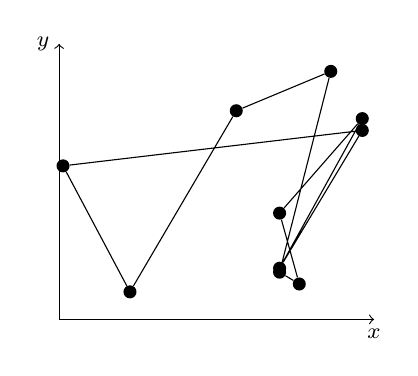
\begin{tikzpicture}[yscale=0.05,xscale=0.05]

      \setcounter{i}{1}

      \draw[->] (0,0) -- (80,0) node[below] {$x$};
      \draw[->] (0,0) -- (0,70) node[left] {$y$};

      \foreach \p in {(18, 7),(1, 39),(77, 48),(56, 13),(77, 51),(56, 27),(61, 9),(56, 12),(69, 63),(45, 53)} {
        \node[point] (\arabic{i}) at \p {};
        \stepcounter{i}
      }

      \draw (1) -- (2) -- (3) -- (4) -- (5) -- (6) -- (7) -- (8) -- (9) -- (10)
      -- (1);
    \end{tikzpicture}
    \caption{Example point cloud used as a polygon with 10 points}
    \label{fig:rcpc:points-10}
  \end{minipage}\hfill
  \begin{minipage}[t]{0.4\textwidth}
    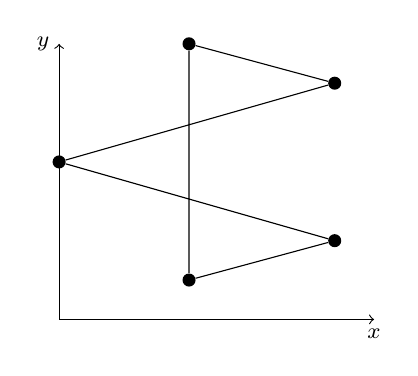
\begin{tikzpicture}[yscale=0.05,xscale=0.05]

      \setcounter{i}{1}

      \draw[->] (0,0) -- (80,0) node[below] {$x$};
      \draw[->] (0,0) -- (0,70) node[left] {$y$};

      \foreach \p in {(70,60), (33,70), (33,10), (70, 20), (0,40)} {
        \node[point] (\arabic{i}) at \p {};
        \stepcounter{i}
      }

      \draw (1) -- (2) -- (3) -- (4) -- (5) -- (1);
    \end{tikzpicture}
    \caption{Example point cloud used as a polygon with 5 points}
    \label{fig:rcpc:points-2}
  \end{minipage}
\end{figure}

\FloatBarrier

\subsection{Regular Polygon}
\subsubsection{Description of the Algorithm}
The main idea behind this algorithm is to rotate a vector around a point
\textit{n} times.

Following a detailed description of the algorithm:

\begin{enumerate}
  \item calculate the parameters
  \item from 1 .. node\_counts calculate the points
  \item reverse the order of points
\end{enumerate}

\subsubsection{Implementation description}
The calculation of the parameters is the first part to do. The
parameter characterize the regular polygon about the position on the
sampling grid, the radius, the winding number and the node count.
There is room for further improvements or more parameters, like to
set the segment length and calculate the possible radius and the
center.

Trigonometric functions like Sinus and Cosinus helps to calculate the points.

\begin{lstlisting}[basicstyle=\scriptsize]
  auto gamma = 2 * \pi * winding_number / node_count;
  auto rotation_angle = -gamma / 2;

  auto x = radius * std::cos(seg_counter * gamma + rotation_angle) + center.x();
  auto y = radius * std::sin(seg_counter * gamma + rotation_angle) + center.y();
\end{lstlisting}

The rotation angle is not necessary for the algorithm. But it helps to perform
calculations during other algorithms easier. The rotation angle $ - gamma / 2$
rotates the whole polygon in a way, that the first segment lies vertically.

The final step revers the order of the points. This is also not really necessary
for the algorithm, but it produces a polygon which has the same direction as the
polygons from all other algorithms.

\subsubsection{Complexity}
The $n$ in the complexity analysis stands for the node count.

\begin{enumerate}
  \item calculate the parameters $\bigO(1)$
  \item from 1 .. node\_counts calculate the points $\bigO(n)$
  \item reverse the order of points $\bigO(n)$
\end{enumerate}

This leads to the sum of $\bigO(1) + \bigO(n) + \bigO(n) \Rightarrow \bigO(n)$


\subsubsection{Parameters}
\begin{description}
  \item [--nodes] how many nodes the polygon has to have. [default: 100]
  \item [--sampling-grid] the area within the polygon could grow. [default: 1500x800]
  %% \item [--winding-number]
  \item [--segment-length] set the segment length. [default: 0]
  \item [--radius] the radius for regular polygon. [default: 60]
\end{description}

\subsubsection{Examples}
\begin{figure}[ht]
  \centering

  \begin{minipage}[t]{0.4\textwidth}
    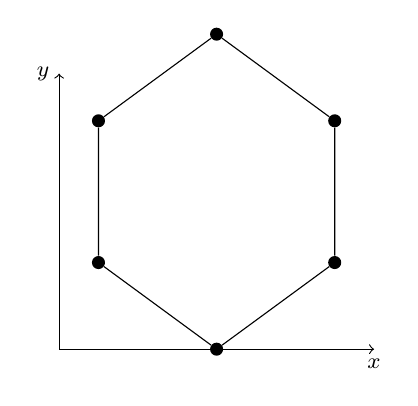
\begin{tikzpicture}[yscale=0.05,xscale=0.05]

      \setcounter{i}{1}

      \draw[->] (0,0) -- (80,0) node[below] {$x$};
      \draw[->] (0,0) -- (0,70) node[left] {$y$};

      \foreach \p in {(40,80), (70,58), (70, 22), (40,0), (10,22), (10,58)} {
        \node[point] (\arabic{i}) at \p {};
        \stepcounter{i}
      }

      \draw (1) -- (2) -- (3) -- (4) -- (5) -- (6) -- (1);
    \end{tikzpicture}
    \caption{Regular polygon with 6 points}
    \label{fig:rp:points-6}
  \end{minipage}\hfill
  \begin{minipage}[t]{0.4\textwidth}
    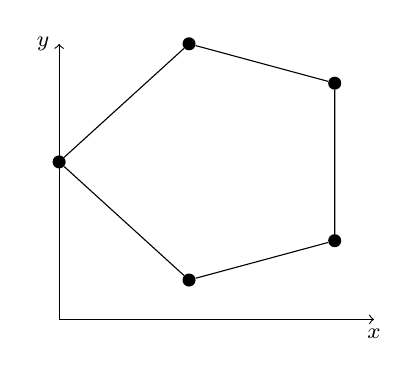
\begin{tikzpicture}[yscale=0.05,xscale=0.05]

      \setcounter{i}{1}

      \draw[->] (0,0) -- (80,0) node[below] {$x$};
      \draw[->] (0,0) -- (0,70) node[left] {$y$};

      \foreach \p in {(33,70), (70,60), (70, 20), (33,10), (0,40)} {
        \node[point] (\arabic{i}) at \p {};
        \stepcounter{i}
      }

      \draw (1) -- (2) -- (3) -- (4) -- (5) -- (1);
    \end{tikzpicture}
    \caption{Regular polygon with 5 points}
    \label{fig:rp:points-5}
  \end{minipage}
\end{figure}

\FloatBarrier

\subsection{Fix Local Orientation}
\subsubsection{Description of the Algorithm}
This algorithm has two steps. The first step is the creation of a regular
polygon. The second step is to include reflex nodes into the segments.
\\[12pt]
Following the description of the algorithm in detail:

\begin{enumerate}
  \item calculate the settings
  \item create the regular polygon
  \item create the reflex nodes
\end{enumerate}

\subsubsection{Implementation description}
A implementation detail in advance. It is helpfull that the regular
polygon algorithm creates a polygon where the first segment lies on a
vertical line, because only than the middle point could be calculated
in a simple way. It is not mandatory but it makes this algorithm easier to
implement.

\begin{enumerate}
  \item calculate the settings with the parameter given by the user or
    the default values. It is important to pay attention that the node count for
    the regular polygon is the node count set by the parameter \textit{--node}
    minus the reflex node count. This part creates also a random list how many
    reflex nodes has to be created in how many segments.
  \item the implementation of the regular polygon algorithm creates the regular
    polygon.
  \item the idea is to create the reflex nodes on the semi circle between the
    segment endpoints. This ensures not any intersection between any segment.
    Following a detailed description of this algorithm:
    \begin{enumerate}
      \item calculate the point in the middle of the first segment and
        the distance from the center to it.
      \item iterate over the segments
      \item wherever reflex nodes have to be added the vector to the
        middle point rotates about the angle from the first segment
        to the current segment to get the position of the middle point
        of the current segment.
      \item calculate the vector \textit{l} from the center of the current
        segment to the target point of the current segment.
      \item with the reflex node counts for this segment and the angle for every
        segment of the regular polygon it could be calculated the angle with
        which the vector \textit{l} could be rotated.
      \item then every reflex node is only a further rotation of the
        vector l.
    \end{enumerate}
\end{enumerate}

\subsubsection{Complexity}
$n$ stands for the node count and $k$ for the maximum possible reflex count per segment.
\begin{enumerate}
  \item calculate the settings $\bigO(1)$
  \item create the regular polygon $\bigO(n)$
  \item create the reflex nodes $\bigO(nk)$
\end{enumerate}
This leads to the sum of $\bigO(1) + \bigO(n) + \bigO(nk) \Rightarrow
max(\bigO(1) + \bigO(n) + \bigO(nk)) \Rightarrow \bigO(nk) \Rightarrow
\bigO(n)$. The value of $k$ and $n$ sums up to the number of nodes given by the
commandline argument. Therefore if $k << n$ then it is a constant factor which
apply every iteration. If $n << k$ then it is the same as before but in opposite
direction which leads to the same result. The last case is, if $k < n, k == n, k
> n$. This means, that if all reflex nodes where set to one segment than all
other segments have nothing to do and if all segments have one reflex node it is
again a constant factor.

\subsubsection{Parameters}
\begin{description}
  \item [--nodes] how many nodes the polygon has to have. [default: 100]
  \item [--sampling-grid] the area within the polygon could grow. [default: 1500x800]
  \item [--reflex-points] set the number of reflex points that should be at least. [default: 0]
  \item [--reflex-chain-max] the maximal length of a chain. the default value says that there is no limit. [default: -1]
  \item [--segment-length] set the segment length. [default: 0]
  \item [--radius] the radius for regular polygon. [default: 60]
\end{description}


\subsubsection{Examples}

\begin{figure}[ht]
  \centering

  \begin{minipage}[t]{0.4\textwidth}
    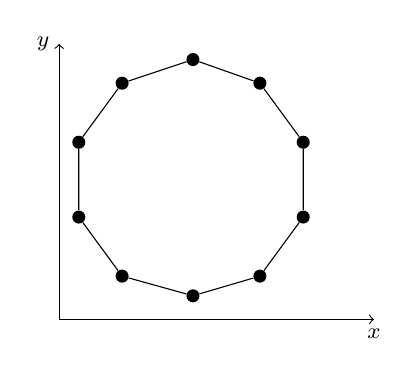
\begin{tikzpicture}[yscale=0.05,xscale=0.05]

      \setcounter{i}{1}

      \draw[->] (0,0) -- (80,0) node[below] {$x$};
      \draw[->] (0,0) -- (0,70) node[left] {$y$};

      \foreach \p in {(62,26),(51,11),(34,6),(16,11),(5,26),(5,45),(16,60),(34,66),(51,60),(62,45)} {
        \node[point] (\arabic{i}) at \p {};
        \stepcounter{i}
      }

      \draw (1) -- (2) -- (3) -- (4) -- (5) -- (6) -- (7) -- (8) -- (9) -- (10) -- (1);
    \end{tikzpicture}
    \caption{Polygon with convex nodes generated by the regular
      polygon algorithm}
    \label{fig:flo:base}
  \end{minipage}\hfill
  \begin{minipage}[t]{0.4\textwidth}
    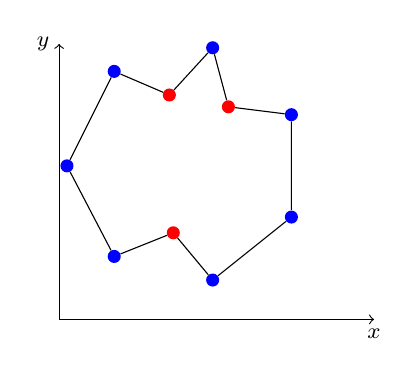
\begin{tikzpicture}[yscale=0.05,xscale=0.05]

      \setcounter{i}{1}

      \draw[->] (0,0) -- (80,0) node[below] {$x$};
      \draw[->] (0,0) -- (0,70) node[left] {$y$};

      \foreach \p in {(59,26),(39,10),(14,16),(2,39),(14,63),(39,69),(59,52)} {
        \node[point,color=blue] (\arabic{i}) at \p {};
        \stepcounter{i}
      }

      \foreach \p in {(29,22),(28,57),(43,54)} {
        \node[point,color=red] (\arabic{i}) at \p {};
        \stepcounter{i}
      }

      \draw (1) -- (2) -- (8) -- (3) -- (4) -- (5) -- (9) -- (6) -- (10) -- (7) -- (1);
    \end{tikzpicture}
    \caption{Regular polygon filled up with reflex nodes[Reflex nodes
    red, convex nodes blue]}
    \label{fig:flo:line}
  \end{minipage}
\end{figure}

\FloatBarrier


\pagebreak

\section{Algorithms bound to point cloud}
The following algorithms starts the calculation of the simple
polygon with a randomly created point cloud.

\begin{enumerate}
  \item Random Two Peasants
  \item Convex Bottom
  \item Steady Growth
  \item Space Partitioning
  \item 2-Opt Moves
\end{enumerate}

\subsection{Random Two Peasants}
\subsubsection{Description of the Algorithm}
The main idea for the random two peasants algorithm is to sort the points along
a axis. The algorithm start from a random 2d point cloud \fref{rtp:base}

\begin{enumerate}
  \item sort all points along the x-axis.
  \item use the line \fref{rtp:line} from lowest point to greatest point
    on x-axis to divide the points in a upper \fref{rtp:upper} and a lower
    \fref{rtp:lower} point cloud.
  \item add sequential all points from the upper list to the polygon
    \fref{rtp:polygon-upper}
  \item add in reverse order all points from the lower list to the
    polygon \fref{rtp:polygon}
\end{enumerate}

\subsubsection{Implementation description}

\begin{enumerate}
  \item the function std::sort from the std lib does the sorting
  \item iterate over all points and perform the CGAL::orientation function to
    get the orientation of all points aligned at the line between the lowest
    point and the highest point.
  \item iterate over all points from the upper list and add it to the polygon
  \item iterate over all points from the lower list in reverse direction and add
    it to the polygon.
\end{enumerate}

\subsubsection{Complexitiy}

\begin{enumerate}
  \item sort all points along the x-axis. $\bigO(nlogn)$
  \item use the line from lowest point to greatest point on x-axis to divide the
    points in a upper and a lower point cloud. $\bigO(n)$
  \item add sequential all points from the upper list to the polygon $\bigO(n)$
  \item add in reverse order all points from the lower list to the polygon $\bigO(n)$
\end{enumerate}

This leads to $max(\bigO(nlogn) + \bigO(n) + \bigO(n) + \bigO(n) \Rightarrow \bigO(nlogn))$.

\subsubsection{Parameters}
\begin{description}
  \item [--nodes] how many nodes the polygon has to have. [default: 100]
  \item [--sampling-grid] the area within the polygon could grow. [default: 1500x800]
\end{description}

\subsubsection{Examples}

\begin{figure}[ht]
  \centering

  \begin{minipage}[t]{0.4\textwidth}
    \begin{tikzpicture}[yscale=0.05,xscale=0.05]
      \setcounter{i}{1}

      \draw[->] (0,0) -- (80,0) node[below] {$x$};
      \draw[->] (0,0) -- (0,70) node[left] {$y$};

      \foreach \p in {(1,11),(5,40),(10,20),(21,10),(20,18),(20,41),(33,15),(39,22),(48,9),(55,17),(60,50),(68,19)} {
        \node[point] (\arabic{i}) at \p {};
        \stepcounter{i}
      }
    \end{tikzpicture}
    \caption{Base random point cloud}
    \label{fig:rtp:base}
  \end{minipage}\hfill
  \begin{minipage}[t]{0.4\textwidth}
    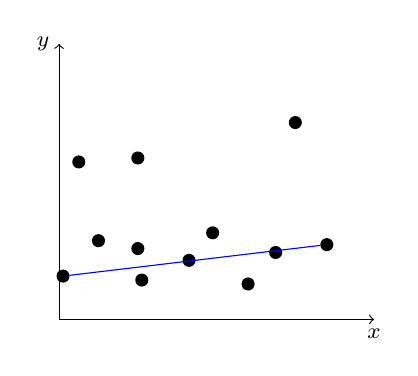
\begin{tikzpicture}[yscale=0.05,xscale=0.05]
      \setcounter{i}{1}

      \draw[->] (0,0) -- (80,0) node[below] {$x$};
      \draw[->] (0,0) -- (0,70) node[left] {$y$};

      \foreach \p in {(1,11),(5,40),(10,20),(21,10),(20,18),(20,41),(33,15),(39,22),(48,9),(55,17),(60,50),(68,19)} {
        \node[point] (\arabic{i}) at \p {};
        \stepcounter{i}
      }

      \draw[blue] (1) -- (12);
    \end{tikzpicture}
    \caption{Dividing Line}
    \label{fig:rtp:line}
  \end{minipage}
\end{figure}

\begin{figure}[ht]
  \centering

  \begin{minipage}[t]{0.4\textwidth}
    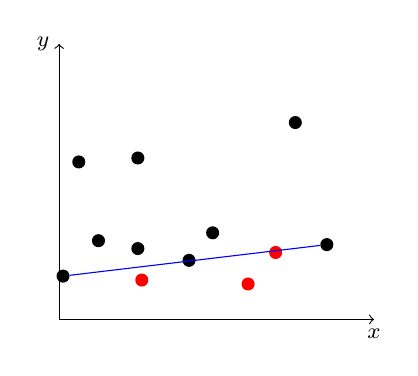
\begin{tikzpicture}[yscale=0.05,xscale=0.05]
      \setcounter{i}{1}

      \draw[->] (0,0) -- (80,0) node[below] {$x$};
      \draw[->] (0,0) -- (0,70) node[left] {$y$};

      \foreach \p in {(1,11),(5,40),(10,20),(20,18),(20,41),(33,15),(39,22),(60,50),(68,19)} {
        \node[point] (\arabic{i}) at \p {};
        \stepcounter{i}
      }

      \foreach \p in {(21,10),(48,9),(55,17)} {
        \node[point, fill=red] (\arabic{i}) at \p {};
        \stepcounter{i}
      }

      \draw[blue] (1) -- (9);
    \end{tikzpicture}
    \caption{Lower List}
    \label{fig:rtp:lower}
  \end{minipage}\hfill
  \begin{minipage}[t]{0.4\textwidth}
    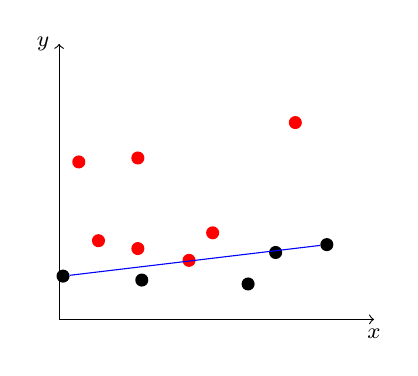
\begin{tikzpicture}[yscale=0.05,xscale=0.05]
      \setcounter{i}{1}

      \draw[->] (0,0) -- (80,0) node[below] {$x$};
      \draw[->] (0,0) -- (0,70) node[left] {$y$};

      \foreach \p in {(1,11),(21,10),(48,9),(55,17),(68,19)} {
        \node[point] (\arabic{i}) at \p {};
        \stepcounter{i}
      }

      \foreach \p in {(5,40),(10,20),(20,18),(20,41),(33,15),(39,22),(60,50)} {
        \node[point, fill=red] (\arabic{i}) at \p {};
        \stepcounter{i}
      }

      \draw[blue] (1) -- (5);
    \end{tikzpicture}
    \caption{Upper list}
    \label{fig:rtp:upper}
  \end{minipage}
\end{figure}

\begin{figure}[ht]
  \centering

  \begin{minipage}[t]{0.4\textwidth}
    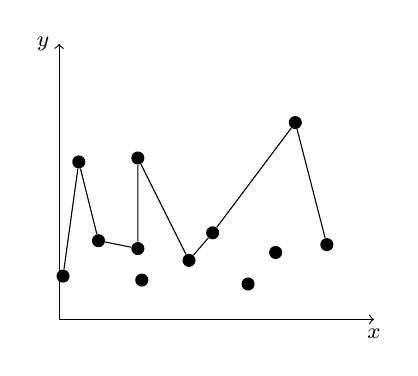
\begin{tikzpicture}[yscale=0.05,xscale=0.05]
      \setcounter{i}{1}

      \draw[->] (0,0) -- (80,0) node[below] {$x$};
      \draw[->] (0,0) -- (0,70) node[left] {$y$};

      \foreach \p in {(1,11),(5,40),(10,20),(21,10),(20,18),(20,41),(33,15),(39,22),(48,9),(55,17),(60,50),(68,19)} {
        \node[point] (\arabic{i}) at \p {};
        \stepcounter{i}
      }
      \draw (1) -- (2) -- (3) -- (5) -- (6) -- (7) -- (8) -- (11) -- (12);
    \end{tikzpicture}
    \caption{The Upper polygon}
    \label{fig:rtp:polygon-upper}
  \end{minipage}\hfill
  \begin{minipage}[t]{0.4\textwidth}
    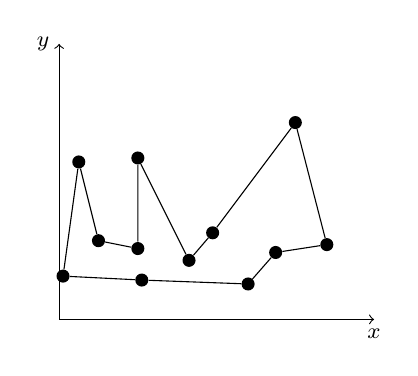
\begin{tikzpicture}[yscale=0.05,xscale=0.05]
      \setcounter{i}{1}

      \draw[->] (0,0) -- (80,0) node[below] {$x$};
      \draw[->] (0,0) -- (0,70) node[left] {$y$};

      \foreach \p in {(1,11),(5,40),(10,20),(21,10),(20,18),(20,41),(33,15),(39,22),(48,9),(55,17),(60,50),(68,19)} {
        \node[point] (\arabic{i}) at \p {};
        \stepcounter{i}
      }

      \draw (1) -- (2) -- (3) -- (5) -- (6) -- (7) -- (8) -- (11) -- (12) -- (10) -- (9) -- (4) -- (1);
    \end{tikzpicture}
    \caption{Final polygon}
    \label{fig:rtp:polygon}
  \end{minipage}
\end{figure}

\FloatBarrier

\subsection{Convex Bottom}
\subsubsection{Description of the Algorithm}
Convex Bottom Algorithm uses the Convex Hull principle to create a convex
polygon. The algorithm starts from a random 2d point cloud.
\fref{cb:base}.
\\[12pt]
Following the description of the algorithm in detail:

\begin{enumerate}
  \item sort all points along the x-axis.
  \item choose the lowest and greatest point on x-axis and draw a line between them\fref{cb:line}
  \item create a list of all points below or on this line \fref{cb:below-line}
  \item create a convex hull from those points \fref{cb:hull}
  \item add points not on the convex bottom hull to the polygon \fref{cb:polygon-1}
  \item add points from the convex bottom hull in reverse order to the polygon
    \fref{cb:polygon-2}
\end{enumerate}

\subsubsection{Implementation description}
\begin{enumerate}
  \item the function std::sort from the std lib does the sorting
  \item the sorted point list gives as the possibility to use the first point
    and the last point as the point with the lowest and the highest x value
  \item the CGAL::orientation function in combination with a for loop checks if
    the point lies below the formed line
  \item the CGAL::convex\_hull\_2 creates the bottom convex hull
  \item add all points which does not lie on the convex bottom hull to the polygon
  \item with std::reverse and a for loop the points from the convex bottom hull
    were added to the final polygon
\end{enumerate}

\subsubsection{Complexity}
\begin{enumerate}
  \item sort all points along the x-axis. $\bigO(nlogn)$
  \item choose the lowest and greatest point on x-axis and draw a line between them $\bigO(1)$
  \item create a list of all points below or on this line $\bigO(n)$
  \item create a convex hull from those points $\bigO(nlogn)$
  \item add points not on the convex bottom hull to the polygon $\bigO(n)$
  \item add points from the convex bottom hull in reverse order to the polygon $\bigO(n)$
\end{enumerate}
In summarize this leads to $\bigO(nlogn)$.

\subsubsection{Parameters}
\begin{description}
  \item [--nodes] how many nodes the polygon have to have. [default: 100]
  \item [--sampling-grid] the area within the polygon could grow. [default: 1500x800]
\end{description}

\subsubsection{Examples}

\begin{figure}[ht]
  \centering

  \begin{minipage}[t]{0.4\textwidth}
    \begin{tikzpicture}[yscale=0.05,xscale=0.05]

      \setcounter{i}{0}

      \draw[->] (0,0) -- (80,0) node[below] {$x$};
      \draw[->] (0,0) -- (0,70) node[left] {$y$};

      \foreach \p in {(1,11),(5,40),(10,20),(21,10),(20,18),(20,41),(33,15),(39,22),(48,9),(55,17),(60,50),(68,19)} {
        \node[point] (\arabic{i}) at \p {};
        \stepcounter{i}
      }
    \end{tikzpicture}
    \caption{Base random point cloud}
    \label{fig:cb:base}
  \end{minipage}\hfill
  \begin{minipage}[t]{0.4\textwidth}
    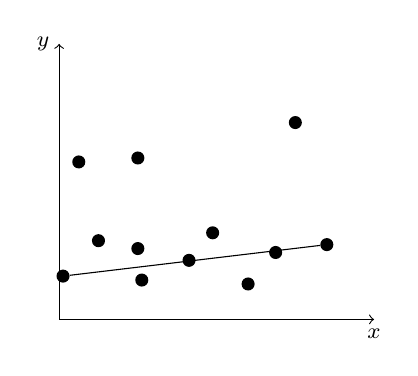
\begin{tikzpicture}[yscale=0.05,xscale=0.05]

      \setcounter{i}{1}

      \draw[->] (0,0) -- (80,0) node[below] {$x$};
      \draw[->] (0,0) -- (0,70) node[left] {$y$};

      \foreach \p in {(1,11),(5,40),(10,20),(21,10),(20,18),(20,41),(33,15),(39,22),(48,9),(55,17),(60,50),(68,19)} {
        \node[point] (\arabic{i}) at \p {};
        \stepcounter{i}
      }

      \draw (1) -- (12);
    \end{tikzpicture}
    \caption{Line from lowest x to highest x}
    \label{fig:cb:line}
  \end{minipage}
\end{figure}

\begin{figure}[ht]
  \centering
  \begin{minipage}[t]{0.4\textwidth}
    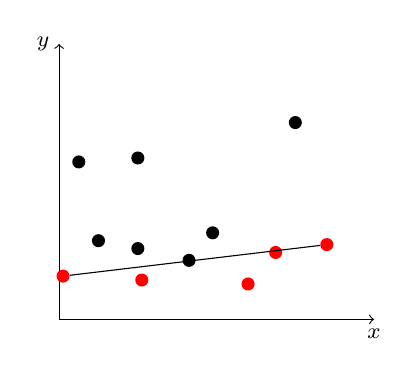
\begin{tikzpicture}[yscale=0.05,xscale=0.05]

      \draw[->] (0,0) -- (80,0) node[below] {$x$};
      \draw[->] (0,0) -- (0,70) node[left] {$y$};

      \node[point, fill=red] (1) at (1,11) {};
      \node[point] (2) at (5,40) {};
      \node[point] (3) at (10,20) {};
      \node[point, fill=red] (4) at (21,10) {};
      \node[point] (5) at (20,18) {};
      \node[point] (6) at (20,41) {};
      \node[point] (7) at (33,15) {};
      \node[point] (8) at (39,22) {};
      \node[point, fill=red] (9) at (48,9) {};
      \node[point, fill=red] (10) at (55,17) {};
      \node[point] (11) at (60,50) {};
      \node[point, fill=red] (12) at (68,19) {};

      \draw (1) -- (12);
    \end{tikzpicture}
    \caption{Points on and below of the line}
    \label{fig:cb:below-line}
  \end{minipage}\hfill
  \begin{minipage}[t]{0.4\textwidth}
    \centering
    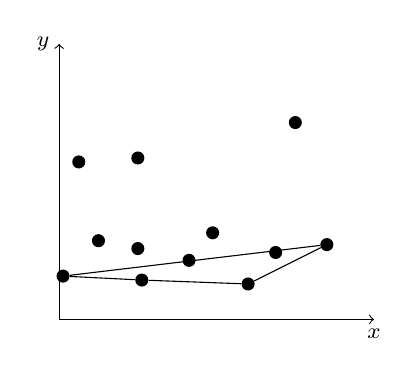
\begin{tikzpicture}[yscale=0.05,xscale=0.05]

      \setcounter{i}{1}

      \draw[->] (0,0) -- (80,0) node[below] {$x$};
      \draw[->] (0,0) -- (0,70) node[left] {$y$};

      \foreach \p in {(1,11),(5,40),(10,20),(21,10),(20,18),(20,41),(33,15),(39,22),(48,9),(55,17),(60,50),(68,19)} {
        \node[point] (\arabic{i}) at \p {};
        \stepcounter{i}
      }

      \draw (1) -- (12) -- (9) -- (4) -- (1);
    \end{tikzpicture}
    \caption{Convex bottom hull}
    \label{fig:cb:hull}
  \end{minipage}
\end{figure}

\begin{figure}[ht]
  \centering
  \begin{minipage}[t]{0.4\textwidth}
    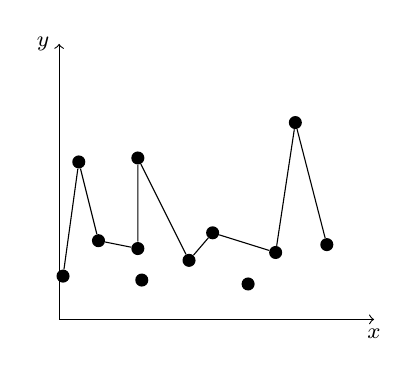
\begin{tikzpicture}[yscale=0.05,xscale=0.05]
      \setcounter{i}{1}

      \draw[->] (0,0) -- (80,0) node[below] {$x$};
      \draw[->] (0,0) -- (0,70) node[left] {$y$};

      \foreach \p in {(1,11),(5,40),(10,20),(21,10),(20,18),(20,41),(33,15),(39,22),(48,9),(55,17),(60,50),(68,19)} {
        \node[point] (\arabic{i}) at \p {};
        \stepcounter{i}
      }

      \draw (1) -- (2) -- (3) -- (5) -- (6) -- (7) -- (8) -- (10) -- (11) -- (12);
    \end{tikzpicture}
    \caption{Polygon from the sorted values}
    \label{fig:cb:polygon-1}
  \end{minipage}\hfill
  \begin{minipage}[t]{0.4\textwidth}
    \centering
    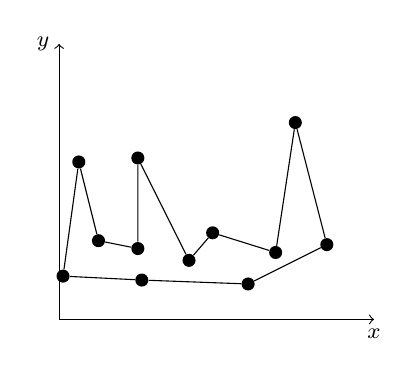
\begin{tikzpicture}[yscale=0.05,xscale=0.05]

      \setcounter{i}{1}

      \draw[->] (0,0) -- (80,0) node[below] {$x$};
      \draw[->] (0,0) -- (0,70) node[left] {$y$};

      \foreach \p in {(1,11),(5,40),(10,20),(21,10),(20,18),(20,41),(33,15),(39,22),(48,9),(55,17),(60,50),(68,19)} {
        \node[point] (\arabic{i}) at \p {};
        \stepcounter{i}
      }
      \draw (1) -- (2) -- (3) -- (5) -- (6) -- (7) -- (8) -- (10) -- (11) -- (12) -- (9) -- (4) -- (1);
    \end{tikzpicture}
    \caption{Polygon from above combined with polygon from below}
    \label{fig:cb:polygon-2}
  \end{minipage}
\end{figure}

\FloatBarrier

\subsection{Steady Growth}
\subsubsection{Description of the Algorithm}
This algorithm is a variation of the convex hull principles. It uses
the convex hull to guarantee that no intersection occurs.
\\[12pt]
Following the description of the algorithm in detail:

\begin{enumerate}
  \item choose two points
  \item initialize polygon and convex hull
  \item randomly iterate over all points
  \begin{enumerate}
    \item the random point has to fulfil one requirement. No remaining, not
      choosen point is allowed to be located within the temporarly extended
      convex hull \fref{sg:point-p}
    \item choose a segment $s$ visible from the point $p$
    \item replace the segment $s$ with the point $p$
    \item add the point $p$ to the convex hull
  \end{enumerate}
\end{enumerate}

\subsubsection{Implementation description}
The above description of the algorithm describes only the theoretical
version of the algorithm. I would like to rewrite the algorithm in a
technical way to have a better entrance to the further description of
the implementation.

\begin{enumerate}
  \item \label{en:sg:a} two points have to be independent from each other
    \fref{sg:line}. They should not lie to far from each other. And they should
    not have another point on the line between them.
  \item \label{en:sg:b} initialize polygon and convex hull
  \item \label{en:sg:c} randomly iterate over all points
  \begin{enumerate}
    \item \label{en:sg:d} first we search the support vertices on the convex
      hull \fref{sg:hull-cv1} for the randomly choosen point \fref{sg:point-p}.
      Then it is necessary to iterate over all points that are not in the
      just constructed polygon. This iteration is necessary to verify that no
      other point lies within the temporarly created convex hull from the old
      convex hull plus the new point. If there is a point within, the support
      vertices has to be recalculated. If a point is found it is
      not necessary to iterate over the already iterated points, because these
      points could only lie outside of the new area.
    \item \label{en:sg:e}to choose a visible segment it is necessary
      to calculate a list of visible segments. First there were
      located all points between the support vertices. With this
      points and the point $p$ it is created a list of segments that
      form a closed polygon. This polygon is necessary to compute the
      visible points from the point $p$. This computation leads to a
      list of points. This points \fref{sg:reg-points} and the points
      calculated before \fref{sg:prob-vis-points} are merged to get
      segments which are completelly visible from point $p$ \fref{sg:vis-seg}.
      This list is used to choose a visible segment.
    \item \label{en:sg:f}for the replacement it is helpfull to know the segment
      on the polygon
    \item \label{en:sg:g}finally the point $p$ is added to the convex hull
  \end{enumerate}
\end{enumerate}

For \eref{sg:a} it is necessary to keep the points in a clockwise
orientation. To ensure this, there is a check if the x value from the
left point is lower than from the right one. This prevents bugs,
because the whole algorithm works only if we start with a clockwise
orientation.

\eref{sg:b} and \eref{sg:c} are implemented straight forward with a
pointlist initialization and a for-loop.

The \eref{sg:d} was difficult. It seems easy but it wasn't. The idea
is to start from the nearest point on the convex hull to the point $p$.
Then iterate right to the point where the polygon from $p$ to $u$ to $v$
doesn't form a right turn. The same in the left direction, where the
polygon from $p$ to $u$ to $v$ should form a left turn. A special case is if the
convex hull consists only of two elements. This is shorter, but the
left turn check has to be done, because of the clockwise direction. If
the check is not done, than the left and right support vertices are
assigned possibly in the wrong order. The nearest point is found by an
algorithmus that checks the intersection between the segment from the
point $p$ to the first point on the convex hull and moving segment from
first point of the hull to the second point of the hull. If such a
intersection occurs than the target is the nearest point. The first
point is used for testing purpose possibility. With the two found
support vertices it is not finished. For all points on the remaining
point list it has the be checked, that no other point lies within the
triangle of left and right support vertices and point $p$. To check this
the cgal function \textit{has\_on\_bounded\_side} from the triangle
class was used. If a point exists then the support
vertices have to be recalculated. This part could be done with minimal
effort, because it is only necessary to iterate forward from the left
support vertices to check against a right turn and from right support
vertices iterate backward and check against left turn. This could be
done in $\bigO{n}$ because processed points could only lie outside of
the possible new triangle.

The main part of \eref{sg:e} is done by the visibility algorithm
implemented by cgal. This algorithm returns a list of points that are
on the polygon and visible from point $p$. Those points does not
necessarily correspond with the points on the polygon. To get the real
visible segments it is necessary to iterate over both point lists.
Three cases exists.

\begin{enumerate}
  \item the next reg (+1) could be a visible point. or
    that the segment is on the line from $p$ to the point $p+1$
  \item after next reg (+2) could be the visible point
  \item after after next reg (+3) could be equal to a visible point
\end{enumerate}

\subsubsection{Complexity}
The complexity is $\bigO(n^2)$

\subsubsection{Parameters}
\begin{description}
  \item [--nodes] how many nodes the polygon has to have. [default: 100]
  \item [--sampling-grid] the area within the polygon could grow. [default: 1500x800]
\end{description}

\subsubsection{Examples}
\begin{figure}[ht]
  \centering

  \begin{minipage}[t]{0.4\textwidth}
    \begin{tikzpicture}[yscale=0.05,xscale=0.05]

      \setcounter{i}{0}

      \draw[->] (0,0) -- (80,0) node[below] {$x$};
      \draw[->] (0,0) -- (0,70) node[left] {$y$};

      \foreach \p in {(1,11),(5,40),(10,20),(21,10),(20,18),(20,41),
        (33,15),(39,22),(48,9),(55,17),(60,50),(68,19)} {
        \node[point] (\arabic{i}) at \p {};
        \stepcounter{i}
      }
    \end{tikzpicture}
    \caption{Base random point cloud}
    \label{fig:sg:base}
  \end{minipage}\hfill
  \begin{minipage}[t]{0.4\textwidth}
    \begin{tikzpicture}[yscale=0.05,xscale=0.05]

      \setcounter{i}{1}

      \draw[->] (0,0) -- (80,0) node[below] {$x$};
      \draw[->] (0,0) -- (0,70) node[left] {$y$};

      \foreach \p in {(1,11),(5,40),(10,20),(21,10),(20,18),(20,41),
        (33,15),(39,22),(48,9),(55,17),(60,50),(68,19)} {
        \node[point] (\arabic{i}) at \p {};
        \stepcounter{i}
      }

      \draw (7) -- (8);
    \end{tikzpicture}
    \caption{Two independent points}
    \label{fig:sg:line}
  \end{minipage}
\end{figure}

\begin{figure}[ht]
  \centering

  \begin{minipage}[t]{0.4\textwidth}
    \begin{tikzpicture}[yscale=0.05,xscale=0.05]

      \setcounter{i}{1}

      \draw[->] (0,0) -- (80,0) node[below] {$x$};
      \draw[->] (0,0) -- (0,70) node[left] {$y$};

      \foreach \p in {(1,11),(5,40),(10,20),(21,10),(20,18),(20,41),
        (33,15),(39,22),(48,9),(55,17),(60,50),(68,19)} {
        \node[point] (\arabic{i}) at \p {};
        \stepcounter{i}
      }

      \draw (7) -- (8);
      \node at (7) [below] {$s_r$};
      \node at (8) [above] {$s_l$};
      \node at (9) [right] {$p$};
    \end{tikzpicture}
    \caption{Point $p$}
    \label{fig:sg:point-p}
  \end{minipage}\hfill
  \begin{minipage}[t]{0.4\textwidth}
    \begin{tikzpicture}[yscale=0.05,xscale=0.05]

      \setcounter{i}{1}

      \draw[->] (0,0) -- (80,0) node[below] {$x$};
      \draw[->] (0,0) -- (0,70) node[left] {$y$};

      \foreach \p in {(1,11),(5,40),(10,20),(21,10),(20,18),(20,41),
        (33,15),(39,22),(48,9),(55,17),(60,50),(68,19)} {
        \node[point] (\arabic{i}) at \p {};
        \stepcounter{i}
      }

      \draw (7) -- (8) -- (9) -- (7);
    \end{tikzpicture}
    \caption{Point $p$ added}
    \label{fig:sg:point-p-add}
  \end{minipage}
\end{figure}

\begin{figure}[ht]
  \centering

  \begin{minipage}[t]{0.4\textwidth}
    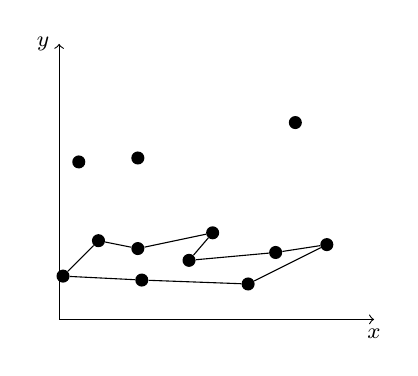
\begin{tikzpicture}[yscale=0.05,xscale=0.05]

      \setcounter{i}{1}

      \draw[->] (0,0) -- (80,0) node[below] {$x$};
      \draw[->] (0,0) -- (0,70) node[left] {$y$};

      \foreach \p in {(1,11),(5,40),(10,20),(20,18),(20,41),(21,10),
        (33,15),(39,22),(48,9),(55,17),(60,50),(68,19)} {
        \node[point] (\arabic{i}) at \p {};
        \stepcounter{i}
      }

      \draw (1) -- (3) -- (4) -- (8) -- (7) -- (10) -- (12) -- (9) -- (6) -- (1);
    \end{tikzpicture}
    \caption{Polygon PY1}
    \label{fig:sg:polygon-py1}
  \end{minipage}\hfill
  \begin{minipage}[t]{0.4\textwidth}
    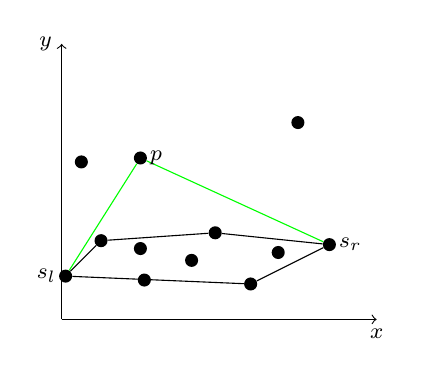
\begin{tikzpicture}[yscale=0.05,xscale=0.05]

      \setcounter{i}{1}

      \draw[->] (0,0) -- (80,0) node[below] {$x$};
      \draw[->] (0,0) -- (0,70) node[left] {$y$};

      \foreach \p in {(1,11),(5,40),(10,20),(20,18),(20,41),(21,10),
        (33,15),(39,22),(48,9),(55,17),(60,50),(68,19)} {
        \node[point] (\arabic{i}) at \p {};
        \stepcounter{i}
      }

      \draw (1) -- (3) -- (8) -- (12) -- (9) -- (1);
      \draw[green] (1) -- (5) -- (12);
      \node at (1) [left] {$s_l$};
      \node at (12) [right] {$s_r$};
      \node at (5) [right] {$p$};
    \end{tikzpicture}
    \caption{Convex Hull CV1 + support vertices}
    \label{fig:sg:hull-cv1}
  \end{minipage}
\end{figure}

\begin{figure}[ht]
  \centering

  \begin{minipage}[t]{0.4\textwidth}
    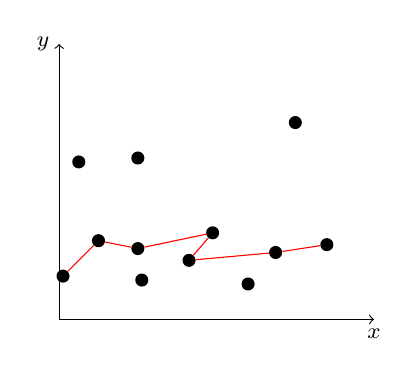
\begin{tikzpicture}[yscale=0.05,xscale=0.05]

      \setcounter{i}{1}

      \draw[->] (0,0) -- (80,0) node[below] {$x$};
      \draw[->] (0,0) -- (0,70) node[left] {$y$};

      \foreach \p in {(1,11),(5,40),(10,20),(20,18),(20,41),(21,10),
        (33,15),(39,22),(48,9),(55,17),(60,50),(68,19)} {
        \node[point] (\arabic{i}) at \p {};
        \stepcounter{i}
      }

      \draw[red] (1) -- (3) -- (4) -- (8) -- (7) -- (10) -- (12);
    \end{tikzpicture}
    \caption{Probably visible points}
    \label{fig:sg:prob-vis-points}
  \end{minipage}\hfill
  \begin{minipage}[t]{0.4\textwidth}
    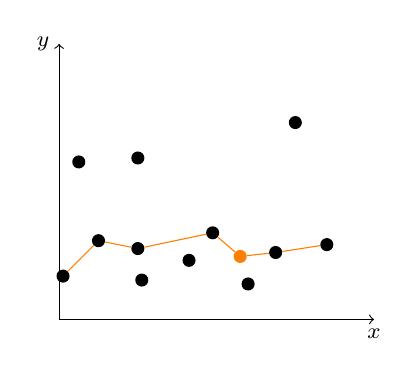
\begin{tikzpicture}[yscale=0.05,xscale=0.05]

      \setcounter{i}{1}

      \draw[->] (0,0) -- (80,0) node[below] {$x$};
      \draw[->] (0,0) -- (0,70) node[left] {$y$};

      \foreach \p in {(1,11),(5,40),(10,20),(20,18),(20,41),(21,10),
        (33,15),(39,22),(48,9),(55,17),(60,50),(68,19)} {
        \node[point] (\arabic{i}) at \p {};
        \stepcounter{i}
      }

      \node[point, orange] (13) at (46,16) {};

      \draw[orange] (1) -- (3) -- (4) -- (8) -- (13) -- (10) -- (12);

    \end{tikzpicture}
    \caption{Regular Points}
    \label{fig:sg:reg-points}
  \end{minipage}
\end{figure}



\begin{figure}[ht]
  \centering

  \begin{minipage}[t]{0.4\textwidth}
    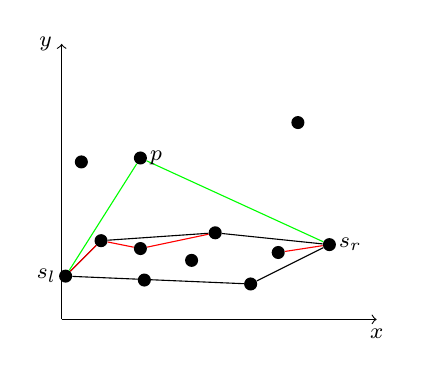
\begin{tikzpicture}[yscale=0.05,xscale=0.05]

      \setcounter{i}{1}

      \draw[->] (0,0) -- (80,0) node[below] {$x$};
      \draw[->] (0,0) -- (0,70) node[left] {$y$};

      \foreach \p in {(1,11),(5,40),(10,20),(20,18),(20,41),(21,10),
        (33,15),(39,22),(48,9),(55,17),(60,50),(68,19)} {
        \node[point] (\arabic{i}) at \p {};
        \stepcounter{i}
      }

      \draw (1) -- (3) -- (8) -- (12) -- (9) -- (1);
      \draw[red] (1) -- (3) -- (4) -- (8);
      \draw[red] (10) -- (12);
      \draw[green] (1) -- (5) -- (12);
      \node at (1) [left] {$s_l$};
      \node at (12) [right] {$s_r$};
      \node at (5) [right] {$p$};
    \end{tikzpicture}
    \caption{Complete Visible Segments (red) from Point $p$}
    \label{fig:sg:vis-seg}
  \end{minipage}\hfill
  \begin{minipage}[t]{0.4\textwidth}
    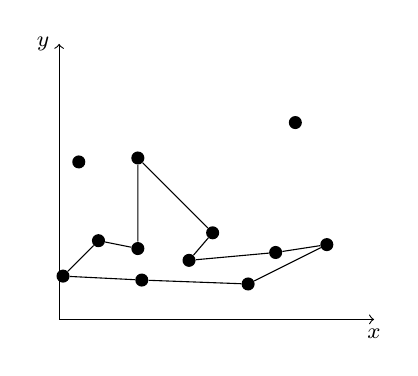
\begin{tikzpicture}[yscale=0.05,xscale=0.05]

      \setcounter{i}{1}

      \draw[->] (0,0) -- (80,0) node[below] {$x$};
      \draw[->] (0,0) -- (0,70) node[left] {$y$};

      \foreach \p in {(1,11),(5,40),(10,20),(20,18),(20,41),(21,10),
        (33,15),(39,22),(48,9),(55,17),(60,50),(68,19)} {
        \node[point] (\arabic{i}) at \p {};
        \stepcounter{i}
      }

      \draw (1) -- (3) -- (4) --(5) -- (8) -- (7) -- (10) -- (12) -- (9) -- (6) -- (1);

    \end{tikzpicture}
    \caption{Polygon PY2}
    \label{fig:sg:polygon-py2}
  \end{minipage}
\end{figure}

\begin{figure}[ht]
  \centering

  \begin{minipage}[t]{0.4\textwidth}
    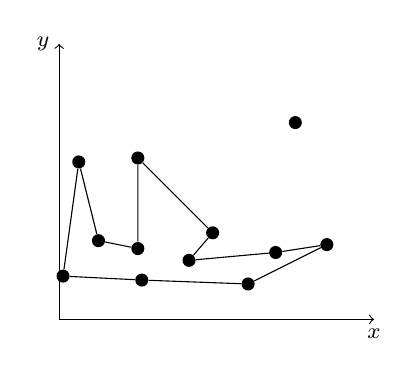
\begin{tikzpicture}[yscale=0.05,xscale=0.05]

      \setcounter{i}{1}

      \draw[->] (0,0) -- (80,0) node[below] {$x$};
      \draw[->] (0,0) -- (0,70) node[left] {$y$};

      \foreach \p in {(1,11),(5,40),(10,20),(20,18),(20,41),(21,10),
        (33,15),(39,22),(48,9),(55,17),(60,50),(68,19)} {
        \node[point] (\arabic{i}) at \p {};
        \stepcounter{i}
      }

      \draw (1) -- (2) -- (3) -- (4) --(5) -- (8) -- (7) -- (10) -- (12) -- (9) -- (6) -- (1);
    \end{tikzpicture}
    \caption{Possible next step}
    \label{fig:sg:polygon-py3}
  \end{minipage}\hfill
  \begin{minipage}[t]{0.4\textwidth}
    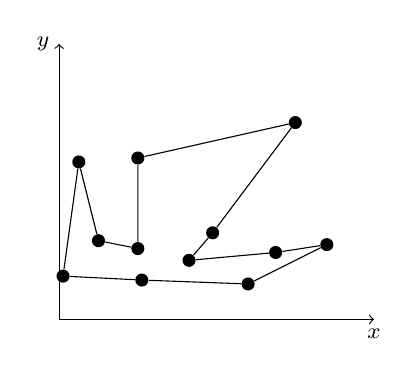
\begin{tikzpicture}[yscale=0.05,xscale=0.05]

      \setcounter{i}{1}

      \draw[->] (0,0) -- (80,0) node[below] {$x$};
      \draw[->] (0,0) -- (0,70) node[left] {$y$};

      \foreach \p in {(1,11),(5,40),(10,20),(20,18),(20,41),(21,10),
        (33,15),(39,22),(48,9),(55,17),(60,50),(68,19)} {
        \node[point] (\arabic{i}) at \p {};
        \stepcounter{i}
      }

      \draw (1) -- (2) -- (3) -- (4) --(5) -- (11) -- (8) -- (7) -- (10) -- (12) -- (9) -- (6) -- (1);
    \end{tikzpicture}
    \caption{Possible last step}
    \label{fig:sg:polygon-py4}
  \end{minipage}
\end{figure}

\FloatBarrier

\subsection{Space Partitioning}
\subsubsection{Description of the Algorithm}
The main idea is a combination of the divide and conquer principle and
the convex hull. The algorithm divides the point cloud by a line and
recursively process those sets. Finally the points of the sets were
pushed to the polygon. The fact that every set has a convex hull that
has only one point in common with adjacent sets guarantees a simple
polygon.
\\[12pt]
Following a description of the algorithm in detail:

\begin{enumerate}
  \item select two points
  \item divide the point cloud by a line through those points \fref{sp:line}
  \item recursively process those two sets of points \fref{sp:line2} to \fref{sp:line5}
  \begin{enumerate}
    \item exit point set of points == 2 || == 3 push points on the final list
    \item calculate a random point
    \item calculate a random line with this point
    \item divide the point cloud by that line
  \end{enumerate}
\end{enumerate}

\subsubsection{Implementation description}
\begin{enumerate}
  \item a random function selects two points ($s_l$ and $s_f$). Point $s_l$ is the
    first point in rotation direction and $s_f$ the second point.
  \item to divide the point cloud in two independent sets we create a
    line through the two points. The \textit{Line\_2} class from the cgal
    framework has a \textit{has\_on\_positive} and \textit{has\_on\_negative} function.
    With these it is possible to distinguish between a point of one or
    the other side of the line.
  \item with the created sets we call recursivelly the function
    \textit{recursiveDivide} and give the function the created set $S$, point $s_f$,
    point $s_l$ and the polygon $C$. One call has as first element $s_f$ the other has $s_l$
    as first element of the two points. This is necessary to close the
    polygon.
  \begin{enumerate}
    \item there are two exit points of the \textit{recursiveDivide} function.
      The first is with set \textit{S.size == 2} and pushs the point $s_l$ to the
      polygon $C$. The second is with set \textit{S.size == 3}. Here we have to
      search the third point $s$, which is not $s_l$ or $s_f$ and then we
      could push $s$ and $s_l$ to the polygon $C$.
    \item if the exit points does not occure we calculate a random
      point. The random point should be selected randomly. The
      condition is that it is not a point equal to and not collinear
      with $s_f$ and $s_l$. The next step is to calculate a random line
      through the point s and a point of the line through $s_f$ and
      $s_l$. Essentially is that $s_f$ lies on the positive side of the
      calculated random line.
    \item the division of the set is equal as in the parent function
  \end{enumerate}
\end{enumerate}

\subsubsection{Complexity}
$\bigO(n^2)$ if it is done in a good way then it should be $\bigO(nlogn)$

\subsubsection{Parameters}
\begin{description}
  \item [--nodes] how many nodes the polygon has to have. [default: 100]
  \item [--sampling-grid] the area within the polygon could grow. [default: 1500x800]
\end{description}

\subsubsection{Examples}

\begin{figure}[ht]
  \centering

  \begin{minipage}[t]{0.4\textwidth}
    \begin{tikzpicture}[yscale=0.05,xscale=0.05]
      \setcounter{i}{1}

      \draw[->] (0,0) -- (80,0) node[below] {$x$};
      \draw[->] (0,0) -- (0,70) node[left] {$y$};

      \foreach \p in {(5,40),(10,20),(20,41),(21,10),(33,15),(39,22),(48,9),(55,17),(68,19)} {
        \node[point] (\arabic{i}) at \p {};
        \stepcounter{i}
      }
    \end{tikzpicture}
    \caption{Base random point cloud}
    \label{fig:sp:base}
  \end{minipage}\hfill
  \begin{minipage}[t]{0.4\textwidth}
    \begin{tikzpicture}[yscale=0.05,xscale=0.05]
      \setcounter{i}{1}

      \draw[->] (0,0) -- (80,0) node[below] {$x$};
      \draw[->] (0,0) -- (0,70) node[left] {$y$};

      \foreach \p in {(5,40),(10,20),(20,41),(21,10)} {
        \node[point, fill=red] (\arabic{i}) at \p {};
        \stepcounter{i}
      }

      \foreach \p in {(33,15),(39,22)} {
        \node[point, fill=violet] (\arabic{i}) at \p {};
        \stepcounter{i}
      }

      \foreach \p in {(48,9),(55,17),(68,19)} {
        \node[point, fill=blue] (\arabic{i}) at \p {};
        \stepcounter{i}
      }

      \path (5) -- (6) coordinate[pos=-3.5](dd) coordinate[pos=10](ff);
      \draw[green, dashed] (dd) -- (5);
      \draw[green] (5) node[right=1pt, black] {$s_f$} -- (6) node[left=1pt, black] {$s_l$};
      \draw[green, dashed] (6) -- (ff);
    \end{tikzpicture}
    \caption{First two points with the line and the two sets. Points on the line are in both sets.}
    \label{fig:sp:line}
  \end{minipage}
\end{figure}

\begin{figure}[ht]
  \centering

  \begin{minipage}[t]{0.4\textwidth}
    \begin{tikzpicture}[yscale=0.05,xscale=0.05]
      \setcounter{i}{1}

      \draw[->] (0,0) -- (80,0) node[below] {$x$};
      \draw[->] (0,0) -- (0,70) node[left] {$y$};

      \foreach \p in {(5,40),(10,20),(20,41),(21,10),(33,15),(39,22),(48,9),(55,17),(68,19)} {
        \node[point] (\arabic{i}) at \p {};
        \stepcounter{i}
      }

      \draw[green] (5) node[right=1pt, black] {$s_f$} -- node[placeholder](a){} (6) node[right=1pt, black] {$s_l$};
      \draw[red] (a) -- (1) node[right=1pt, black] {$s$};
    \end{tikzpicture}
    \caption{First split of left set}
    \label{fig:sp:line2}
  \end{minipage}\hfill
  \begin{minipage}[t]{0.4\textwidth}
    \begin{tikzpicture}[yscale=0.05,xscale=0.05]
      \setcounter{i}{1}

      \draw[->] (0,0) -- (80,0) node[below] {$x$};
      \draw[->] (0,0) -- (0,70) node[left] {$y$};

      \foreach \p in {(5,40),(10,20),(20,41),(21,10),(33,15),(39,22),(48,9),(55,17),(68,19)} {
        \node[point] (\arabic{i}) at \p {};
        \stepcounter{i}
      }

      \draw (5) -- node[placeholder](a){} (6);
      \draw (a) -- node[placeholder](b){} (1);
      \draw (2) -- (b);
    \end{tikzpicture}
    \caption{Second split of left set}
    \label{fig:sp:line3}
  \end{minipage}
\end{figure}

\begin{figure}[ht]
  \centering

  \begin{minipage}[t]{0.4\textwidth}
    \begin{tikzpicture}[yscale=0.05,xscale=0.05]
      \setcounter{i}{1}

      \draw[->] (0,0) -- (80,0) node[below] {$x$};
      \draw[->] (0,0) -- (0,70) node[left] {$y$};

      \foreach \p in {(5,40),(10,20),(20,41),(21,10),(33,15),(39,22),(48,9),(55,17),(68,19)} {
        \node[point] (\arabic{i}) at \p {};
        \stepcounter{i}
      }

      \draw (5) -- node[placeholder](a){} (6);
      \draw (a) -- node[placeholder](b){} (1);
      \draw (2) -- (b);
      \draw (8) -- (a);
    \end{tikzpicture}
    \caption{First split of right set}
    \label{fig:sp:line4}
  \end{minipage}\hfill
  \begin{minipage}[t]{0.4\textwidth}
    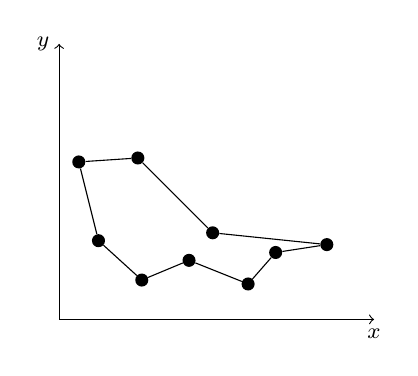
\begin{tikzpicture}[yscale=0.05,xscale=0.05]
      \setcounter{i}{1}

      \draw[->] (0,0) -- (80,0) node[below] {$x$};
      \draw[->] (0,0) -- (0,70) node[left] {$y$};

      \foreach \p in {(5,40),(10,20),(20,41),(21,10),(33,15),(39,22),(48,9),(55,17),(68,19)} {
        \node[point] (\arabic{i}) at \p {};
        \stepcounter{i}
      }

      \draw (5) -- (4) -- (2) -- (1) -- (3) -- (6) -- (9) -- (8) -- (7) -- (5);
    \end{tikzpicture}
    \caption{Final polygon}
    \label{fig:sp:line5}
  \end{minipage}
\end{figure}

\FloatBarrier

\subsection{2-Opt Moves}
\subsubsection{Description of the Algorithm}
The main idea behind this algorithm is to construct the simply polygon
by resolving the intersections.

\begin{enumerate}
  \item create segments from a random polygon
  \item calculate all intersections of segments
  \item iterate over all intersections
	\begin{enumerate}
    \item choose a intersection
    \item remove all intersections where one of the two segments are
      involved
    \item remove the segments from the intersection from the segments
      list
    \item create new segments from those two segments
    \item calculate all intersection that occure by the new segments
    \item add the two segments to the segments list
  \end{enumerate}
  \item calculate the final list of the segments list
\end{enumerate}

\subsubsection{Implementation description}
\begin{enumerate}
  \item the creation of the segments is trivial
  \item the calculation of the intersections consists of two nested
    loops over all segments. The important part is to have no
    duplicates of intersections. This is implemented with a map and a
    duplicate check. The map was choosen because of the O(log(n))
    complexity to search and add elements.
  \begin{enumerate}
    \item the random function chooses the random intersection
    \item a for loop to iterate over the intersections and remove the
      intersections which have one or both segments in common
    \item remove the segments from the segments list with a simple erase from
      the vector class
    \item the creation of the new segments is difficult. The
      difficulty is to reorder the segments in a way that the polygon
      is still closed and does not decay in two independed polygons.
      This is guaranteed by a creation of the polygon, the same as the
      creation of the final polygon and to check if the size is equal
      of the size of the segments list.
    \item the new intersections with the new segments are calculated
      by a loop over all segments and a insert into the intersections
      map.
    \item add the segments to the segments list
  \end{enumerate}
  \item to create the final list of the segments are two loops
    necessary. the first loop builds two maps with a source -> target
    combination as key -> value, both ends of the segments were added
    as key respective value. The second map is necessary because a key
    could be occure twice but only twice and therefore two maps. The
    second loop iterates from 1 to N where N is the number of points
    in the polygon and builds the polygon by moving from source to
    target and to use the old target for the new source.
\end{enumerate}

\subsubsection{Complexity}
The implemented complexity is $\bigO(n^2*log(n))$.

\subsubsection{Parameters}
\begin{description}
  \item [--nodes] how many nodes the polygon has to have. [default: 100]
  \item [--sampling-grid] the area within the polygon could grow. [default: 1500x800]
\end{description}

\subsubsection{Examples}
\begin{figure}[ht]
  \centering

  \begin{minipage}[t]{0.4\textwidth}
    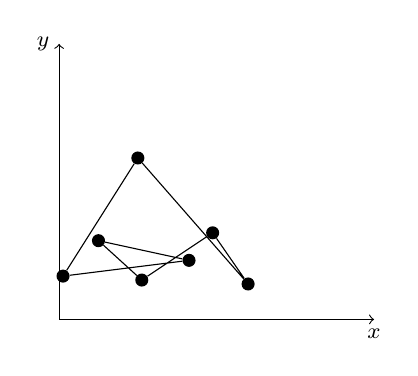
\begin{tikzpicture}[yscale=0.05,xscale=0.05]

      \setcounter{i}{1}

      \draw[->] (0,0) -- (80,0) node[below] {$x$};
      \draw[->] (0,0) -- (0,70) node[left] {$y$};

      \foreach \p in {(1,11),(33,15),(10,20),(21,10),(39,22),(48,9),(20,41)} {
        \node[point] (\arabic{i}) at \p {};
        \stepcounter{i}
      }

      \draw (1) -- (2) -- (3) -- (4) -- (5) -- (6) -- (7) -- (1);
    \end{tikzpicture}
    \caption{Random polygon}
    \label{fig:tom:base}
  \end{minipage}\hfill
  \begin{minipage}[t]{0.4\textwidth}
    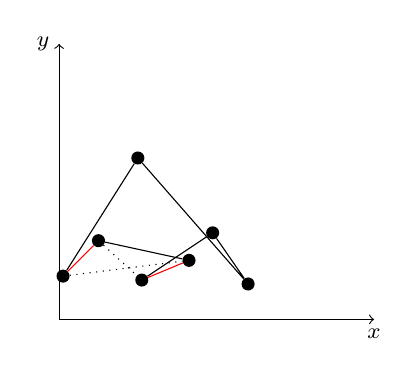
\begin{tikzpicture}[yscale=0.05,xscale=0.05]

      \setcounter{i}{1}

      \draw[->] (0,0) -- (80,0) node[below] {$x$};
      \draw[->] (0,0) -- (0,70) node[left] {$y$};

      \foreach \p in {(1,11),(33,15),(10,20),(21,10),(39,22),(48,9),(20,41)} {
        \node[point] (\arabic{i}) at \p {};
        \stepcounter{i}
      }

      \draw[dotted] (1) -- (2);
      \draw[dotted] (3) -- (4);
      \draw[red] (1) -- (3);
      \draw[red] (2) -- (4);
      \draw (2) -- (3);
      \draw (4) -- (5) -- (6) -- (7) -- (1);
    \end{tikzpicture}
    \caption{First step of resolving}
    \label{fig:tom:res1}
  \end{minipage}
\end{figure}

\begin{figure}[ht]
  \centering

  \begin{minipage}[t]{0.4\textwidth}
    \begin{tikzpicture}[yscale=0.05,xscale=0.05]

      \setcounter{i}{1}

      \draw[->] (0,0) -- (80,0) node[below] {$x$};
      \draw[->] (0,0) -- (0,70) node[left] {$y$};

      \foreach \p in {(1,11),(33,15),(10,20),(21,10),(39,22),(48,9),(20,41)} {
        \node[point] (\arabic{i}) at \p {};
        \stepcounter{i}
      }

      \draw[dotted] (2) -- (3);
      \draw[dotted] (4) -- (5);
      \draw[red] (3) -- (4);
      \draw[red] (2) -- (5);
      \draw (1) -- (3);
      \draw (4) -- (2);
      \draw (5) -- (6) -- (7) -- (1);
    \end{tikzpicture}
    \caption{Second step of resolving}
    \label{fig:tom:res2}
  \end{minipage}\hfill
  \begin{minipage}[t]{0.4\textwidth}
    \begin{tikzpicture}[yscale=0.05,xscale=0.05]

      \setcounter{i}{1}

      \draw[->] (0,0) -- (80,0) node[below] {$x$};
      \draw[->] (0,0) -- (0,70) node[left] {$y$};

      \foreach \p in {(1,11),(33,15),(10,20),(21,10),(39,22),(48,9),(20,41)} {
        \node[point] (\arabic{i}) at \p {};
        \stepcounter{i}
      }

      \draw[dotted] (2) -- (5);
      \draw[dotted] (6) -- (7);
      \draw[red] (2) -- (6);
      \draw[red] (5) -- (7);
      \draw (1) -- (3) -- (4) -- (2);
      \draw (6) -- (5);
      \draw (7) -- (1);
    \end{tikzpicture}
    \caption{Third step of resolving}
    \label{fig:tom:res3}
  \end{minipage}
\end{figure}

\begin{figure}[ht]
  \centering

  \begin{minipage}[t]{0.4\textwidth}
    \begin{tikzpicture}[yscale=0.05,xscale=0.05]

      \setcounter{i}{1}

      \draw[->] (0,0) -- (80,0) node[below] {$x$};
      \draw[->] (0,0) -- (0,70) node[left] {$y$};

      \foreach \p in {(1,11),(33,15),(10,20),(21,10),(39,22),(48,9),(20,41)} {
        \node[point] (\arabic{i}) at \p {};
        \stepcounter{i}
      }

      \draw[dotted] (2) -- (5);
      \draw[dotted] (6) -- (7);
      \draw[red] (2) -- (7);
      \draw[red] (5) -- (6);
      \draw (1) -- (3) -- (4) -- (2);
      \draw (7) -- (1);
    \end{tikzpicture}
    \caption{Wrong resolving, because of two reasons. First: two segments exists before. Second: the polygon is not more complete nor simple}
    \label{fig:tom:wrong}
  \end{minipage}\hfill
  \begin{minipage}[t]{0.4\textwidth}
    \begin{tikzpicture}[yscale=0.05,xscale=0.05]

      \setcounter{i}{1}

      \draw[->] (0,0) -- (80,0) node[below] {$x$};
      \draw[->] (0,0) -- (0,70) node[left] {$y$};

      \foreach \p in {(1,11),(33,15),(10,20),(21,10),(39,22),(48,9),(20,41)} {
        \node[point] (\arabic{i}) at \p {};
        \stepcounter{i}
      }

      \draw (1) -- (3) -- (4) -- (2) -- (6) -- (5) -- (7) -- (1);
    \end{tikzpicture}
    \caption{Final simple polygon}
    \label{fig:tom:final}
  \end{minipage}
\end{figure}

\FloatBarrier


\clearpage

\section{Algorithms bound to simple polygon}
The following algorithm needs a simple polygon to work.

\subsection{Bouncing Vertices}
\subsubsection{Description of the algorithm}
The main idea behind Bouncing Vertices is to take a simple polygon and
bounce the points randomly by retaining the simple status. Further, it
is possible to restrict the movement of the bouncing step by certain
requirements. Requirements could be, for example to retain the convex
and/or reflex status of the bouncing point.

\subsubsection{Steps of the algorithm}

The bouncing loop could be achieved in two different ways. Both have been
implemented.

\paragraph{Check after the point is temporarly moved}
\begin{enumerate}
  \item initialize settings
  \item convert point list to segment list
  \item bounce every point n times
  \begin{enumerate}
    \item choose a point inside the sampling grid
    \item if wanted, check if the orientation is still the same
    \item if wanted, check if the angle is still within the given range
    \item check if the moved point causes an intersection
    \item follow the above steps until a point fullfills all of them
  \end{enumerate}
\end{enumerate}

\paragraph{Calculate the allowed segment before moving the point}
\begin{enumerate}
  \item initialize settings
  \item convert point list to segment list
  \item bounce every point n times
  \begin{enumerate}
    \item choose a random angle to move the point
    \item calculate the random line to move the point
    \item calculate allowed segment which is has no intersections with other
      segments or the border
    \item if wanted, calculate allowed segment to keep the angle range for the
      current point and the point before and the point after the current point
    \item if wanted, calculate allowed segment to keep the orientation of the
      current point, the point before and the point after the current point
    \item merge those allowed segments to the smallest allowed segment
    \item choose a random value [0,distance)
    \item move the point to the new position
  \end{enumerate}
\end{enumerate}

\subsubsection{Description of implementation}
This algorithm is straight forward to implement, and also gives the
opportunity to extend the requirements to bounce a point, like the
angle range or the orientation stability.

As mentioned above, the bouncing loop can be done in two different
ways. Both possibilities of implementation are described below.

\paragraph{Check after the point is temporarly moved}

\begin{enumerate}
  \item the initialization of the values succeeds by the
    ``BouncingVerticesSettings'' struct
  \item the conversion from point list to segment list is implemented
    with a ``for loop''
  \item bounce every point n times
  \begin{enumerate}
    \item choose a velocity vector randomly within the range given
      by the bouncing radius parameter within the sampling grid
      boundaries. This is implemented with a do while loop.
    \item to check the orientation stability it is necessary to
      compare the old and the new segments around the bouncing point.
      Three equalities have to be equal: the orientation in the
      bouncing point, the orientation in the point before and the
      orientation in the point after the bouncing point. This is
      necessary because the current point affects the orientation of
      the previous point and next point.
    \item there are two cases to consider when the angle range needs
      to be checked. The first is, if the orientation takes place,
      then the old points have to be used to calculate the necessary
      angle influenced by the old orientation. The second case is, if
      the orientation does not take place, and therefore only the
      angle range is used. To implement this the current segments
      were used to calculate the orientation to choose the necessary
      angle range.
    \item the intersection check is also straight forward implemented.
      a loop to iterate over all segments, and to check if both new
      segments would create a intersection. Some cases have to be
      noted. The checked segment should be different from the old
      segments. If the current segment to check has common starting
      points with the new segments, then it is only checked about
      collinearity which would be interpreted as a intersection.
  \end{enumerate}
\end{enumerate}

\paragraph{Calculate the allowed segment before moving the point}
\begin{enumerate}
  \item the initialization of the values succeeds by the
    BouncingVerticesSettings struct
  \item the convertion from point list to segment list is straight
    forward a for loop
  \item bounce every segment n times
  \begin{enumerate}
    \item the value gets choosen by a random function from [0, 360).
      the whole range could be used except of two values. The angles
      from the next and the previous segment.
    \item create a temporary line and rotate that around the current point
    \item calculate the intersection with the sampling\_grid. then iterate over
      all segments and check if there are intersections and if the distance to
      the bouncing point is lower. Update the allowed segment if necessary
    \item to keep the angle range it is necessary to do two steps. First the
      allowed segment for the combination of the point before and the point
      after the current point has to be calculated. This is done by rotating the
      line throw the segment before by the angle range and intersect it with the
      random line. This produces 4 allowed segments. These have to be combined
      to two according to the orientation of the points before and after. The
      second step is to calculate the allowed segment according to the angle
      range of the current point. To do this the Thales's Theorem is used. The
      first step is to calculate the bisecting line of the point before A and the
      point after B the current point C. The next step is to create a vector
      from A to B. This vector is rotated according to the angle range. The
      intersection between this vector and the bisecting line is the center of
      the circle in which every line from point A to the circle to point B has
      the angle with which the vector was rotated.
    \item to calculate the allowed segment for the orientation stability it is
      necessary to intersect the prev segment (target is A) and the next segment
      (source is A) with the random line and construct a allowed segment.
    \item merge the allowed segments to find the smallest allowed
    \item calculate the new point by choosing a value $d$ between 0 and distance of
      allowed segment $D$. calculate the point by $d/D * A + (1-d/D) * B$
  \end{enumerate}
\end{enumerate}


\subsubsection{Complexity}
\paragraph{Check after the point is temporarly moved}
\begin{enumerate}
  \item initialize settings $\bigO(1)$
  \item convert point list to segment list $\bigO(n)$
  \item bounce every segment n times $\bigO(n)$
  \begin{enumerate}
    \item choose a point inside the sampling grid $\bigO(P(x = point\ inside\ grid))$
    \item if wanted check if the orientation is still the same $\bigO(1)$
    \item if wanted check if the angle is still in given range $\bigO(1)$
    \item check if the moved point cause a intersection $\bigO(n)$
    \item do the above steps until a point fullfills all of them $\bigO(k)$
  \end{enumerate}
\end{enumerate}
The complexity depends with this implementation a little on the
probabilty how fast a correct point is found. Otherwise every point
has to be bounced for a fixed count of phases. On every iteration
every segment has to be checked of intersection, therefore
$\bigO(n^2*k)$ should be the complexity. n is the number of points, k
is the number how often a new point has to be choosen to fullfill the
requirements. This value depends on the parameter set to restrict the
valid area.

\paragraph{Calculate the allowed segment before moving the point}
\begin{enumerate}
  \item initialize settings $\bigO(1)$
  \item convert point list to segment list $\bigO(n)$
  \item bounce every segment n times $\bigO(n)$
  \begin{enumerate}
    \item all calculation have $\bigO(1)$
    \item the intersection part has $\bigO(n)$
  \end{enumerate}
\end{enumerate}

This leads to $\bigO(n^2)$

\subsubsection{Parameters}
\begin{description}
  \item [--nodes] how many nodes the polygon have to have. [default: 100]
  \item [--sampling-grid] the area within the polygon could grow. [default: 1500x800]
  \item [--phases] how many phases a random algorithm should run. [default: 10]
  \item [--bouncing-radius] the distance to move a random point from old to new point. [default: 60]
  \item [--animation] create a animation of the different phases of bouncing vertices. default is 0 for false, to start the creation set this to 1. [default: 0]
  \item [--out-every-phase] to output every phase as a gnuplot file. [default: 0]
  \item [--reflex-points] set the number of reflex points that should be at least. [default: 0]
  \item [--reflex-angle-range] set the range of the reflex angle. the angle is interpreted as open in mathematical sense (180..360). [default: 180..360]
  \item [--convex-angle-range] set the range of the convex angle. the angle is interpreted as open in mathematical sense (0..180). [default: 0..180]
\end{description}

\subsubsection{Examples}
\begin{figure}[ht]
  \centering

  \begin{minipage}[t]{0.4\textwidth}
    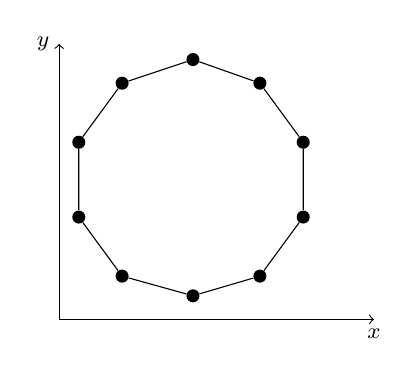
\begin{tikzpicture}[yscale=0.05,xscale=0.05]

      \setcounter{i}{1}

      \draw[->] (0,0) -- (80,0) node[below] {$x$};
      \draw[->] (0,0) -- (0,70) node[left] {$y$};

      \foreach \p in {(62,26),(51,11),(34,6),(16,11),(5,26),(5,45),(16,60),(34,66),(51,60),(62,45)} {
        \node[point] (\arabic{i}) at \p {};
        \stepcounter{i}
      }

      \draw (1) -- (2) -- (3) -- (4) -- (5) -- (6) -- (7) -- (8) -- (9) -- (10) -- (1);
    \end{tikzpicture}
    \caption{Regular Polygon. Startpoint for the algorithm}
    \label{fig:bv:base}
  \end{minipage}\hfill
  \begin{minipage}[t]{0.4\textwidth}
    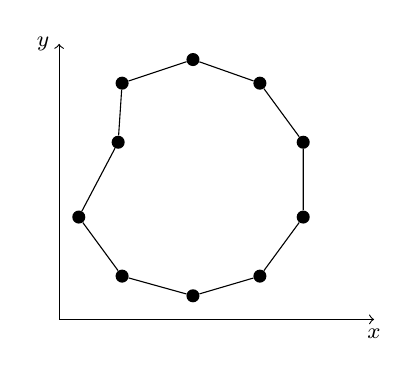
\begin{tikzpicture}[yscale=0.05,xscale=0.05]

      \setcounter{i}{1}

      \draw[->] (0,0) -- (80,0) node[below] {$x$};
      \draw[->] (0,0) -- (0,70) node[left] {$y$};

      \foreach \p in {(62,26),(51,11),(34,6),(16,11),(5,26),(15,45),(16,60),(34,66),(51,60),(62,45)} {
        \node[point] (\arabic{i}) at \p {};
        \stepcounter{i}
      }

      \draw (1) -- (2) -- (3) -- (4) -- (5) -- (6) -- (7) -- (8) -- (9) -- (10) -- (1);
    \end{tikzpicture}
    \caption{Point 6 has moved}
    \label{fig:bv:bounce2}
  \end{minipage}
\end{figure}

\begin{figure}[ht]
  \centering

  \begin{minipage}[t]{0.4\textwidth}
    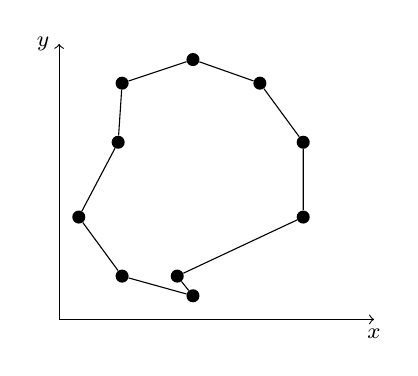
\begin{tikzpicture}[yscale=0.05,xscale=0.05]

      \setcounter{i}{1}

      \draw[->] (0,0) -- (80,0) node[below] {$x$};
      \draw[->] (0,0) -- (0,70) node[left] {$y$};

      \foreach \p in {(62,26),(30,11),(34,6),(16,11),(5,26),(15,45),(16,60),(34,66),(51,60),(62,45)} {
        \node[point] (\arabic{i}) at \p {};
        \stepcounter{i}
      }

      \draw (1) -- (2) -- (3) -- (4) -- (5) -- (6) -- (7) -- (8) -- (9) -- (10) -- (1);
    \end{tikzpicture}
    \caption{Point 3 has moved}
    \label{fig:bv:bounce3}
  \end{minipage}\hfill
  \begin{minipage}[t]{0.4\textwidth}
    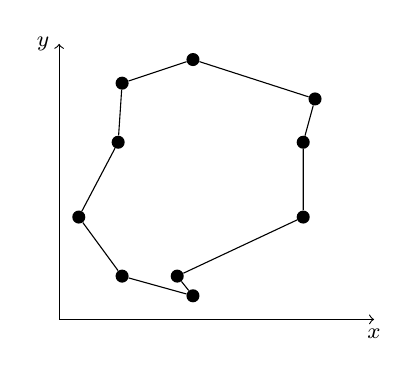
\begin{tikzpicture}[yscale=0.05,xscale=0.05]

      \setcounter{i}{1}

      \draw[->] (0,0) -- (80,0) node[below] {$x$};
      \draw[->] (0,0) -- (0,70) node[left] {$y$};

      \foreach \p in {(62,26),(30,11),(34,6),(16,11),(5,26),(15,45),(16,60),(34,66),(65,56),(62,45)} {
        \node[point] (\arabic{i}) at \p {};
        \stepcounter{i}
      }

      \draw (1) -- (2) -- (3) -- (4) -- (5) -- (6) -- (7) -- (8) -- (9) -- (10) -- (1);
    \end{tikzpicture}
    \caption{Point 9 has moved}
    \label{fig:bv:bounce4}
  \end{minipage}
\end{figure}

\begin{figure}[ht]
  \centering

  \begin{minipage}[t]{0.4\textwidth}
    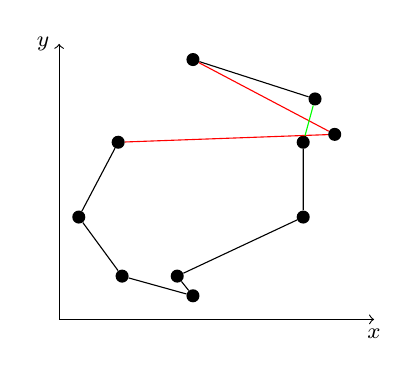
\begin{tikzpicture}[yscale=0.05,xscale=0.05]

      \setcounter{i}{1}

      \draw[->] (0,0) -- (80,0) node[below] {$x$};
      \draw[->] (0,0) -- (0,70) node[left] {$y$};

      \foreach \p in {(62,26),(30,11),(34,6),(16,11),(5,26),(15,45),(70,47),(34,66),(65,56),(62,45)} {
        \node[point] (\arabic{i}) at \p {};
        \stepcounter{i}
      }

      \draw (1) -- (2) -- (3) -- (4) -- (5) -- (6);
      \draw (10) -- (1);
      \draw (8) -- (9);
      \draw[red] (6) -- (7) -- (8);
      \draw[green] (9) -- (10);
    \end{tikzpicture}
    \caption{The red lines cut the green line, which is not good, and not valid!}
    \label{fig:bv:bounce5}
  \end{minipage}\hfill
  \begin{minipage}[t]{0.4\textwidth}
    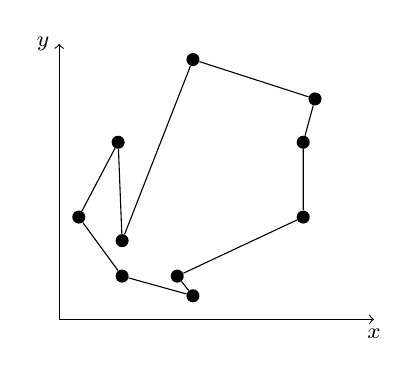
\begin{tikzpicture}[yscale=0.05,xscale=0.05]

      \setcounter{i}{1}

      \draw[->] (0,0) -- (80,0) node[below] {$x$};
      \draw[->] (0,0) -- (0,70) node[left] {$y$};

      \foreach \p in {(62,26),(30,11),(34,6),(16,11),(5,26),(15,45),(16,20),(34,66),(65,56),(62,45)} {
        \node[point] (\arabic{i}) at \p {};
        \stepcounter{i}
      }

      \draw (1) -- (2) -- (3) -- (4) -- (5) -- (6) -- (7) -- (8) -- (9) -- (10) -- (1);
    \end{tikzpicture}
    \caption{Valid movement!}
    \label{fig:bv:bounce6}
  \end{minipage}
\end{figure}


\begin{figure}[ht]
  \begin{tikzpicture}[yscale=0.2,xscale=0.2]
    \setcounter{i}{1}

    \draw[->] (0,0) -- (80,0) node[below] {$x$};
    \draw[->] (0,0) -- (0,70) node[left] {$y$};

    \foreach \p in {(10,10),(30,10),(30,30),(10,30)} {
      \node[point] (\arabic{i}) at \p {};
      \stepcounter{i}
    }

    \draw (1) -- (2) -- (3) -- (4) -- (1);

    \node (5) at (0,20) {};
    \node (6) at (20,0) {};
    \draw (5) -- (6);
  \end{tikzpicture}
  \caption{first test}
\end{figure}

\newcommand{\axis}{
  \draw[->] (0,0) -- (13,0) node[below] {$x$};
  \draw[->] (0,0) -- (0,10) node[left] {$y$};
}

\newcommand{\polygon}[1]{
  \draw[name path=polygon]
    \foreach \x [count=\xi] in {#1} {
      \x node[point] (node\xi) {}
    }

    \foreach \x [count=\xi, remember=\xi-1 as \xiprev] in {#1} {
      \ifnum\xi>1%
        (node\xiprev) -- (node\xi)
      \fi
    }
  ;
}

\newcommand{\randomLine}[4]{
  \ifthenelse{\equal{#3}{}}{
    \draw[name path=randomLine,rotate=0] #1 -- #2;
  }{
    \draw[name path=randomLine,rotate around={#3:#4}] #1 -- #2;
  }
}

\newcommand{\intersection}[2]{
  \fill[red, name intersections={of=#1 and #2, total=\t}]
    \foreach \s in {1,...,\t}{(intersection-\s) circle (5pt) node{\s}};
}

\begin{figure}[ht]
  \begin{tikzpicture}[yscale=0.75,xscale=0.75]
    \axis
    \polygon{(2,2),(3,4),(9,6),(12,1),(8,2),(5,1),(2,2)}
    \randomLine{(5,0)}{(5,7)}{}{}
    \intersection{randomLine}{polygon}
  \end{tikzpicture}
  \caption{intersection free with vertical line}
\end{figure}

\begin{figure}[ht]
  \begin{tikzpicture}[yscale=0.75,xscale=0.75]
    \axis
    \polygon{(2,2),(3,4),(9,6),(12,1),(8,2),(5,1),(2,2)}
    \randomLine{(0,2)}{(13,2)}{}{}
    \intersection{randomLine}{polygon}
  \end{tikzpicture}
  \caption{intersection free with horizontal line}
\end{figure}

\begin{figure}[ht]
  \begin{tikzpicture}[yscale=0.75,xscale=0.75]
    \axis
    \polygon{(2,2),(3,4),(9,6),(12,1),(8,2),(5,1),(2,2)}
    \randomLine{(0,2)}{(13,2)}{30}{(8,2)}
    \intersection{randomLine}{polygon}
  \end{tikzpicture}
  \caption{intersection free with slightly rotated line}
\end{figure}

\begin{figure}[ht]
  \begin{tikzpicture}[yscale=0.75,xscale=0.75]
    \axis
    \polygon{(2,2),(3,4),(9,6),(12,1),(8,2),(5,1),(2,2)}
    \randomLine{(5,0)}{(5,7)}{}{}

    \draw[red, shorten >=-3cm, shorten <= -3cm] (2,2) -- (3,4);
    \draw[red, shorten >=-3cm, shorten <= -3cm] (2,2) -- (8,2);
    \draw[red, shorten >=-3cm, shorten <= -3cm] (12,1) -- (8,2);

    %% \intersection{randomLine}{reflexLine}
    %% \intersection{randomLine}{convexLine}
  \end{tikzpicture}
  \caption{orientation stability with vertical line}
\end{figure}

\begin{figure}[ht]
  \begin{tikzpicture}[yscale=0.35,xscale=0.35]
    \draw[->] (0,0) -- (40,0) node[below] {$x$};
    \draw[->] (0,0) -- (0,40) node[left] {$y$};
    \polygon{(23.7135,28.4134), (21.5339, 25.4134), (18.0072,24.2675), (14.4805,25.4134), (12.3009, 28.4134), (12.3009, 32.1216), (14.4805, 35.1216), (18.0072, 36.2675), (21.5339, 35.1216), (23.7135,32.1216),(23.7135,28.4134)}
    \randomLine{(18.5339, 25.4134)}{(38.5339, 25.4134)}{128.25}{(21.5339, 25.4134)}
    \intersection{randomLine}{polygon}
  \end{tikzpicture}
  \caption{intersection free with slightly rotated line}
\end{figure}

\begin{figure}[ht]
  \begin{tikzpicture}[yscale=0.25,xscale=0.25]
    \draw[->] (0,0) -- (70,0) node[below] {$x$};
    \draw[->] (0,0) -- (0,70) node[left] {$y$};
    \polygon{(20,30),(20,50),(30,60),(50,60),(60,50),(60,30),(28,24),(30,20),(20,30)}
    \randomLine{(-10,20)}{(70,20)}{-30}{(30,20)}
    %%\intersection{randomLine}{polygon}
    \draw[shorten >=-6cm] (20,30) -- (28,24);
  \end{tikzpicture}
  \caption{intersection free with slightly rotated line}
\end{figure}


\FloatBarrier


\end{document}
